
\section{Evaluation}
\label{sec:eval}

In this section, we will compare the performance of original LibFuzzer, our LibFuzzer and AFL. We use fuzzer-test-suite, a set of tests for fuzzing engines provided by Google, as the test cases. In order to support our LibFuzzer, we modify the \texttt{target.cc} in some test cases. Take \texttt{c-ares-CVE-2016-5180} for example, we modified the \texttt{extern "C" int LLVMFuzzerTestOneInput(const uint8\_t *Data, size\_t Size)} function declaration to \texttt{int main()}. And use \texttt{read} function to read input data, the size is the length of input data. Check out more detail of patching fuzzer-test-suite in wiki page of our repository. The following specification is our machine information and all experiments were performed on it.

\begin{lstlisting}
virtual private server on Google Cloud Platform
n1-standard-1 (one vCPU, 3.75 GB RAM)
\end{lstlisting}

\subsection{Compared with original LibFuzzer}

We choose some CVE test cases in fuzzer-test-suite, including \texttt{CVE-2016-5180}, \texttt{CVE-2015-8317} and \texttt{HeartBleed (CVE-2014-0160)}, to evaluate the performance of our LibFuzzer. These are the output of running test cases by our LibFuzzer.

\begin{enumerate}
    \item [1.] \texttt{CVE-2016-5180}
    \begin{lstlisting}
    #0      READ units: 1
    #2      INITED cov: 4 ft: 20 corp: 1/1b exec/s: 2 rss: 25Mb
    #3      NEW    cov: 4 ft: 39 corp: 2/3b exec/s: 3 rss: 25Mb L: 2/2 MS: 1 CopyPart-
    #4      pulse  cov: 4 ft: 59 corp: 2/3b exec/s: 2 rss: 25Mb
    #4      NEW    cov: 4 ft: 59 corp: 3/5b exec/s: 2 rss: 25Mb L: 2/2 MS: 2 CopyPart-ShuffleBytes-
    Error status : 139
    Signal : Segmentation fault
    \end{lstlisting}

    \item [2.] \texttt{CVE-2015-8317}
    \begin{lstlisting}
    #0      READ units: 1
    Error status : 139
    Signal : Segmentation fault
    \end{lstlisting}

    \item [3.] \texttt{HeartBleed (CVE-2014-0160)}
    \begin{lstlisting}
    #0      READ units: 1
     WARNING : block size exceeding max block size at 0x004959e0
    [+] Try changing it with e anal.bb.maxsize
     WARNING : block size exceeding max block size at 0x004d7920
    [+] Try changing it with e anal.bb.maxsize
     WARNING : block size exceeding max block size at 0x0043e9d0
    [+] Try changing it with e anal.bb.maxsize
     WARNING : block size exceeding max block size at 0x0043f160
    [+] Try changing it with e anal.bb.maxsize
     WARNING : block size exceeding max block size at 0x004962f0
    [+] Try changing it with e anal.bb.maxsize
     WARNING : block size exceeding max block size at 0x00496e70
    [+] Try changing it with e anal.bb.maxsize
     WARNING : block size exceeding max block size at 0x00457460
    [+] Try changing it with e anal.bb.maxsize
     WARNING : block size exceeding max block size at 0x004f2ace
    [+] Try changing it with e anal.bb.maxsize
    Error status : 134
    Signal : Aborted
    \end{lstlisting}

\end{enumerate}

Compared with original LibFuzzer and plot the chart.

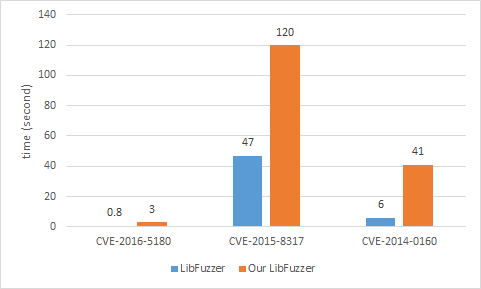
\includegraphics[width=\linewidth]{eval1.png}

As we can see, because the implementaion of our LibFuzzer, the IO speed and analysis take a lot of time. And the preformance is slower than original LibFuzzer. But compared the time of original LibFuzzer and our LibFuzzer took, we still can find the bugs efficiently in these test cases.

\subsection{Compared with AFL}


